\documentclass[aps,prl,reprint,nobalancelastpage,nofootinbib]{revtex4-2}
\usepackage[utf8]{inputenc}
\usepackage{amsmath}
\usepackage{amssymb}
\usepackage{tikz}
\usetikzlibrary{calc}
\usepackage{xcolor}
\usepackage[framemethod=tikz]{mdframed}

\begin{document}

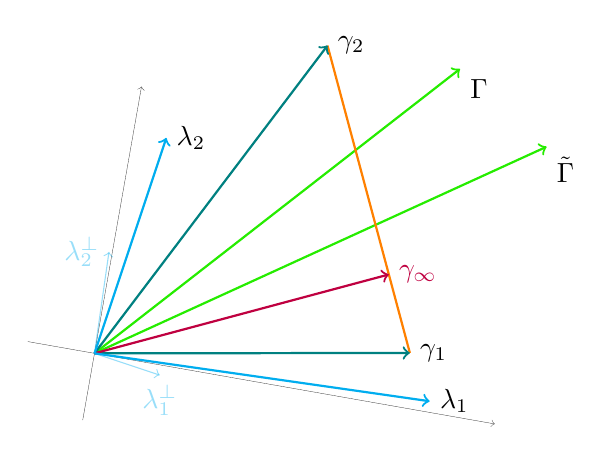
\begin{tikzpicture}[xscale=0.86,yscale=0.86,every node/.style={font=\normalsize},rotate=15]

\begin{scope}[rotate=-25]
    \draw[->,ultra thin,opacity=0.85] (-1,0) -- (6,0);
    \draw[->,ultra thin,opacity=0.85] (0,-1) -- (0,4);

        \draw[->, thick, green!85!orange] (0,0) -- (4.586,5.074) node[below right,black]{$\Gamma$};
        \draw[->, thick, green!85!orange] (0,0) -- (6.045,4.164) node[below right,black]{$\tilde{\Gamma}$};
\end{scope}

\draw[orange, thick] (4.5,-1.2) -- (4.5,3.5);

\draw[->, thick, teal] (0,0) -- (4.5,-1.2) node[right,black]{$\gamma_1$};
\draw[->, thick, teal] (0,0) -- (4.5,3.5) node[right,black]{$\gamma_2$};
\draw[->, thick, purple] (0,0) -- (4.5,0) node[right] {$\gamma_\infty$};

\begin{scope}[rotate=30]

    \draw[->, thick, cyan] (0,0) -- (3,-4) node[right,black]{$\lambda_1$};
    \draw[->, thick, cyan] (0,0) -- (3,3/2) node[right,black]{$\lambda_2$};

    \draw[->, thin, cyan, opacity=0.4] (0,0) -- (5/11,-10/11) node[below]{$\lambda^\perp_1$};
    \draw[->, thin, cyan, opacity=0.4] (0,0) -- (40/33,10/11) node[left]{$\lambda^\perp_2$};

\end{scope}

\end{tikzpicture}

\end{document}